\documentclass[english]{tktltiki}
\usepackage[pdftex]{graphicx}
\usepackage{subfigure}
\usepackage{url}
<<<<<<< HEAD
\usepackage{amsmath}
=======

>>>>>>> 0340f5627ddf9543b5b886b3aa1a82b7b8f7f949
\usepackage[latin9]{inputenc}
\usepackage[]{algorithm2e}

\begin{document}
%\doublespacing
%\singlespacing
\onehalfspacing
\title{Planning Based Computational Narrative With an Emphasis on Surprise Arousal  }
\author{Amin Sorkhei}
%\date{21.09.2014}

\maketitle

\numberofpagesinformation{\numberofpages\ pages + \numberofappendixpages\ appendices}
\classification{}

%\keywords{AI , Minimax Algorithm, \(A^*\) Algorithm, Real Time Strategy games, Planning}

\begin{abstract}
At the galloping rate that computational creativity is flourishing, narrative systems has an important role to play and different computer scientists have tried to come up with methods and approaches in order to create intelligent writers for educational and entraining purposes \cite{planning:2010:NPB:1946417.1946422}. Through the reach history of this newly emerged field, different well known methods like planning based computational narratives have been proposed while this category has been belittled to goal-driven problem-solving aesthetics \cite {analogy}. This short report has as its purpose to propose some general guidelines about computational narratives which are the building blocks of successful systems like MEXICA.
\end{abstract}

\mytableofcontents
\section{Introduction}
As the first step, in order to have systems capable of narrating in a plausible way, some requirements must be satisfied by the system. To put this in other words the methodology and constraints followed by human writers, must be codded to the system. These requirements and constraints are called \textit{'Cognitive Account'}. Additionally, the whole process of writing in human writers can be considered as a cycle of \textit{engagement} and \textit{reflection}. 
\section{Narrative and Planning}
This section provides the reader with some background about both narrative and planning as the foundations of computational narrative. This section embarks on with a quick overview on narrative and what it is composed of.
\subsection{Introduction to Narrative}
<<<<<<< HEAD
Narrative and story-telling are old terms that has an specific role in human history. Since the dawn of human beings, people have tried to transfer their beliefs and ideas and even experiences to the next generation using narratives. On the other hand, psychologists believe that narratives have specific role to play in in pedagogical purposes. While the role of narrative and story-telling is quite appreciated in history, scientists believe that narrative is not well defined. One definition for narrative, proposed in \cite{planning:2010:NPB:1946417.1946422}, is:
\begin{flushleft}
\textit{\textbf{Narrative}: A narrative is the recounting of a sequence of events that have a continuant subject and constitute a whole } 
\end{flushleft}

While this is a general definition regarding narrative and storytelling, we will need a more detailed investigation about what narratives are composed of. Narratologists break the narratigve into two layers of interpretation: \textit{fabula} and \textit{sjuzet}. 

Fabula is the general content of the narrative, loosely speaking, fabula is what the story is going to talk about. On the other hand \textit{sjuzet} is the way the story is going to be presented. To put this in order words, sjuzet decides the order of presentation of events in fabula.To put this in more understandable words, fabula is the raw material of the story while sjuzet determines the way a story is organized. By the way of example, if a narrative is going to talk about the bibliography of a scientist, fabula contains the bibliography of the scientist, while sjuzet specifies the order the story is presented. It can be organized from the time the scientist dies and goes back to his birthday or the other way around. Regardless of which of these sjuzets are preferred, the fabula stays the same. \newline
It is noteworthy to mention that the study focuses mainly on narrative generation in fabula level which is sometimes called \textit{'Fabula Planning Problem'}. Officially Fabula Planning problem is defined as \cite{planning:2010:NPB:1946417.1946422}: 
\begin{flushleft}
\textit{\textbf{Fabula Planning Problem}: Given a domain theory, find a sound and believable sequence of actions that transfer the initial state \textit{I} to a predefined goal state \textit{G} where some conditions are satisfied }
\end{flushleft}
In this definition the domain theory, are a set of actions that change the story world. For example, committing a crime and rain fall are two simple examples of those actions. 
\subsection{Quality of a Narrative}
So far we know what a Narrative and a 'Fabula Planning Problem' is and now we face an important question \textit{'What is a good narrative?'}. \newline
Inherently, audience of a story are inferring machines who try to infer and guess the final result of a story based on the actions performed by characters so far. In other words, human audience constantly, checks how the actions performed by a character are\textit{ believable} and \textit{intentional}. More formally the audience pays attention to character intentionality and believability. Thus, if the audience find the actions committed by a character believable and intentional, the story can be considered as a good one. More importantly, believable and intentional characters bring about a story where human audience can guess the outcome of the story. Definitely, this can not be considered as a good story for people who are fan on surprise in narratives!
As the final word, it is quite acknowledged that believable and intentional actions needs some goal to follow. In other words, believability and intentionality of characters are clearly based on character goals. The important fact which needs to be notices is that, character goals in a story are not necessarily are in the same direction with final goal of the narrative as a whole constitute. To put this in other words, character may have adversarial goals as compared to each other. As an example, a character may want to kill the other character, while the other one wants to strive and live. More importantly, character goals may get resolved and formed during a narrative. As an illustration to this, in some stages of a story one character may prefer to avenge another character, while in future stage they may cultivate friendships due to some sacrifices. 
\subsection{Introduction to planning}
This section provides an overview on planning and presents detailed reasons whether the classic form of planning can be used as a building block for computational narrative or not and finalizes with a brief introduction to customized planning algorithm for narrative generation.\newline 
=======
This section describes \textit{fabula} and \textit{sjuzet}.
Fabula is the general content of the narrative, loosely speaking, fabula is what the story is going to talk about. On the other hand \textit{sjuzet} is the way the story is going to be presented. To put this in oder words, sjuzet decides the order of presentation of events in fabula.
\subsection{planning}
This section tries to provide the reader with an overview on planning and presents detailed reasons whether the classic form of planning can be used a building block for computational narrative or not. More importantly some specific language used in planning for story generation will be presented and finalizes with a brief introduction to customized planning algorithm for narrative generation. 
\subsection{Introduction to planning}
>>>>>>> 0340f5627ddf9543b5b886b3aa1a82b7b8f7f949
Planning--in general terms-- can be considered as one of the well established and old topics in Artificial Intelligence(AI). In the simplest form, through the planning process, intelligent agent tries to come up with a sequence of actions in order to accomplish a predefined goal. Formally planning can be considered using a state-system transition as a 4-tuple $\Sigma = (S,A,E,\gamma)$\newline
$S=\{s_1,s_2,...\}$ is a set of states used to describe the world in a given moment\newline
$A=\{a_1,a_2,...\}$ is a set of actions which can be performed by the agent\newline
$E=\{e_1,e_2,...\}$ is a set of events which can be performed independent of the agent like having an accident.\newline
$\gamma = S\times(A \cup E) \longrightarrow 2^s$ is a transition function which transits the current state of the world based on performed action or observed event. \newline
Trivially for each planning problem, it is required to have a starting state and a goal state where the final goal on the planning can be described as getting started at starting point, executing the planned sequence of actions and reaching the final goal.
Solving 8-tile puzzle can be considered as a simple example of planning problem where actions are moving tiles to the blank area and states are one of the $9!$ possible permutations of tiles. It is noteworthy that in this example, the event set is an empty set.
<<<<<<< HEAD
As the final remark, planning can be divided to partial-order and total order planning. In partial-order some actions can be switched with each other while in the latter form -- total-order planning -- switching actions results in total failure.
=======
As the final remark, planning can be divided to partial-order and total order planning. In partial-order some actions can be switched with each other while in the latter form --total-order planning-- switching actions results in total failure.
>>>>>>> 0340f5627ddf9543b5b886b3aa1a82b7b8f7f949
After this brief introduction to planning, a pivotal question can be whether this general form of planning can be considered as a medium for narrative generation or not. The answer to this question will be investigated in detail through the upcoming sections.
\subsubsection{Customized planning versus classical planning }
As we are familiar with basics of planning, one might consider this off-the-shelf form of planning as the building block of narrative generation. To put this in more details, based on this methodology, each character in the story can be considered as an agent who tries to final accomplish the final goal in the story by doing some actions. This naive idea gives some fundamental ideas about narrative generation while it is too simple to be be deployed to generate narratives.
The most important defect regards this methodology is the fact that, the final goal of the story may be totally different from the goal of each agent (planner). To put this in other words, believable stories are built upon believable characters which in return requires each character to have unique intentions --which may or may not be the same as the final goal of the main plot-- and must perform believable actions justifying the unique goal regarding the character \cite{planning:2010:NPB:1946417.1946422}. As an illustration to this, consider the following plot of a story which is obtained from \cite{planning:2010:NPB:1946417.1946422}:
\begin{flushleft}
<<<<<<< HEAD
\textit{There are three characters in the world, a king,a princess and a knight. All these characters live in castle where there is a tower where each character can be locked up. The final goal of the story is that the princess is locked up in the tower and the king is dead.}'
=======
`\textit{There are three characters in the world, a king,a princess and a knight. All these characters live in castle where there is a tower where each character can be locked up. The final goal of the story is that the princess is locked up in the tower and the king is dead.}'
>>>>>>> 0340f5627ddf9543b5b886b3aa1a82b7b8f7f949
\end{flushleft}
By using the naive idea of using off-the-shelf classical planning algorithm, the following story may be generated
\begin{flushleft}
\textit{1.The princess kills the king \newline 2.The princess locks herself in the tower}
\end{flushleft}
which is not believable to human audience at all, while the plan is totally valid as it starts from the starting position and transforms the world to the goal state where the king is dead and the princess is locked in the tower. From the logical and causal point of view the story does not ring any bell in the human audience to persuade him or her about the intention of the characters. Why does the princess kill the king and why dose she lock herself in the tower. More importantly, is it a believable action for a character to lock him or herself in a place? . Since there is no rationale answer to these questions, the believability and the intentionality of characters is demolished.
The following example depicts a narrative which totally satisfies all the requirements of intentionality and believability of characters as well as reaching the predefined goals.
\begin{flushleft}
\textit{1.The king locks the princess in the tower \newline 2.The knight kills the king}
\end{flushleft} 
<<<<<<< HEAD
In this case, the human reader can easily reason the intentionality of the characters. The princess has done some thing which should have agonized the king and the the king, in return, locked the princess in the tower and the knight kills the king as the revenge. \newline
As the conclusion, for narrative generating purposes, the planning algorithm needs to satisfy the following conditions: \newline
1.The planning algorithm needs to have specific structure for satisfy character intentionality and believability. To put this in other words, it is required to have some events which motivates a character to pursue a specific goal and perform an action. \newline
2. The actions in the domain theory must come in a structure where the participants of an action are determined and precondition and postcondition of an action is specified. In this way a chronological order can be depicted among the actions where the precondition of an action is unified with the post condition of another one.\newline
The upcoming sections talk about \textit{POCL} and \textit{IPOCL} as two specific planning algorithms tuned for narrative generation purposes.
\section{Tuned algorithms for narrative generation}
In this section the provided material and figures are based on \cite{planning:2010:NPB:1946417.1946422}, unless it is specified explicitly.
So far we have got some minimum requirements for algorithms required to perform planning based narrative generation. In this section we get the chance to go through the detail of Partial Order Causal Link (POCL) planner and the refined form, Intent-Driven Partial Order Causal Link (IPOCL) planner.
\subsection{POCL planners}
As mentioned before as one of the requirements for the tuned algorithms, the actions must come in a from where the participants, precondition and effects of actions are specified and stored. In order to do so the actions(operators) are in STRIPS constructs. In STRIPS construct each operator has a name, a precondition -- the condition required for an action to be performed -- and a postcondition which is the effect of the action. Each operator may have variables, which can bound with ground variables to determine the characters engaged in the action. Formally a POCL Plan is defined as:
\begin{flushleft}
\textit{\textbf{POCL Plan}: A POCL plan is a tuple $<S,B,O,L>$ such that $S$ is a set of plan steps(actions),$B$ is a set of bindings constraints on the parameters of the steps in $S$, $O$ is a set of temporal ordering of the form $s_1 < s_2$ where $s_1,s_2 \in S$ and $L$ is a set of causal links of the from $<s_1,p,q,s_2>$ where $s_1,s)2 \in S$ ad $p$ is the effect (postcondition) of $s_1$ and $q$ is the precondition of $s_2$ and $p$ unifies with $q$ }
\end{flushleft}
The are some points need to be elaborated on through the above definition: 
1.As it was mentioned above the terms step, action and operator may be used interchangeably and convey the same meaning. \newline
2. A causal link  connects two steps with a condition $p$ and is written as $s_1 \xrightarrow{p} s_2$ when $s_1$ results in a condition $p$ which is required as a precondition for $s_2$ to execute. \newline

POCL planners try to plan steps in an iterative manner by resolving some flaws at each step. In general terms, flaws are whatever that preclude an answer to be a valid one. More specifically, POCL planners try to resolve two main form of  flaws:
1. \textit{Open condition} flaw: An open condition flaw occurs when a the goal state in the plan is not satisfied, or there is an step like $s_2$ in the plan where its precondition is not satisfied by neither the initial step nor a preceding step like $s_1$. The POCL planners tries to resolve open condition flaw by non-deterministically instantiating a new step or use the existing steps in order to satisfy the required precondition. It means that the planner tries to instantiate a new step or use the existing steps to come up with an action which has a postcondition that unifies with the required precondition or the goal state. In this case causal links of the form can be well used to record the satisfaction of an open flaw and store the dependencies between actions. \newline
2.\textit{Causal threat} flaw: This threat occurs where the effect of a step may undo the effect of another step in the plan. In this case the planner tries to resolve the flaw by explicitly ordering the conflicting flaws \cite{narrativeconflict}.
The following figure contains information about how iteratively POCL planner tries to resolve the flaws.
\begin{figure}[h!]
\centering
	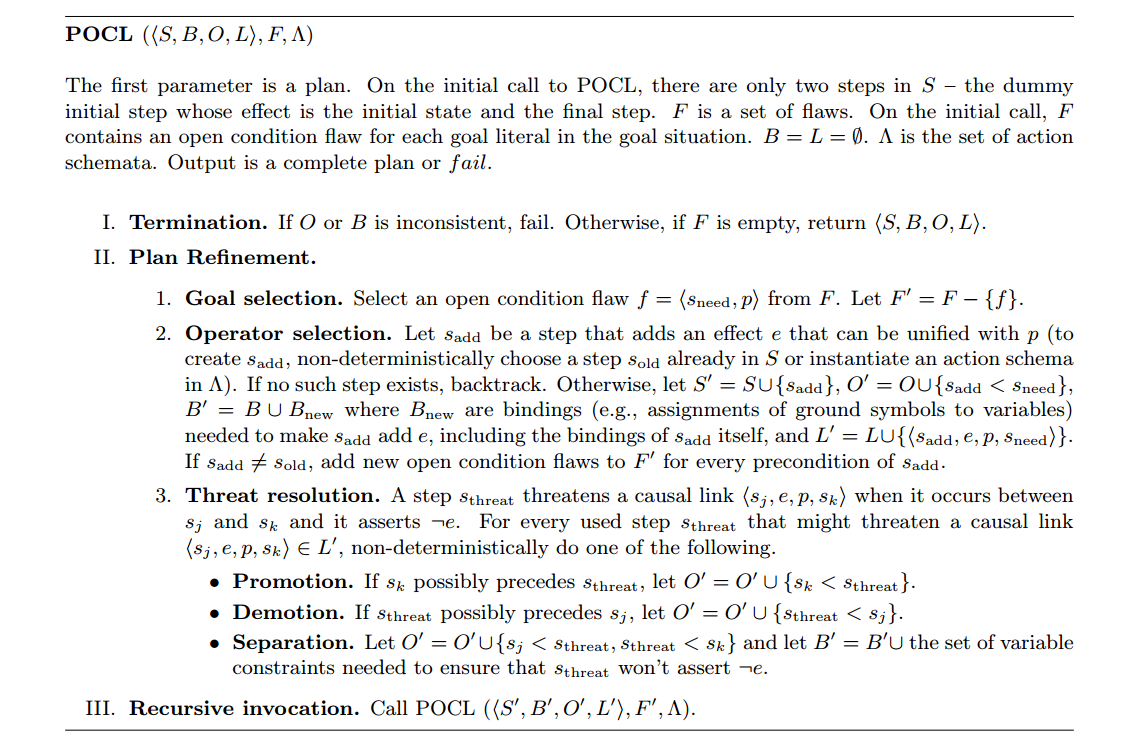
\includegraphics[width=1\textwidth]{POCL}
\caption{POCL algorithm}
\end{figure}
So far we got the chance to get familiar with a powerful variation of planning algorithms where the causal link between the actions are totally guaranteed. In other words, The result of the POCL algorithm is guaranteed to be coherent and actions appear in a logical manner. Here comes up an important question, is POCL the best algorithms that we can deploy?\newline
The answer to this question is negative as POCL provides no way to address the intentionality and believability of characters. To put this in other words, POCL does not provide us with a mechanism to make the story world characters appear intentional. In this case, we need some modification to POCL in order to include some other steps -- called motivating steps -- to make the characters appear intentional and as the result, believable. More importantly, we may need to add some modifications to the construct that is used to present operators. Through the upcoming sections, detail elaboration of the modifications will be presented.
\subsection{IPOCL Planners: First encounter}
As a quick recap, we are dealing with problems where the outcome should be a plan where a wide range of actions are assigned to story world characters. We need each character to be intentional , which means that we need them to pursue individual goals, where individual goal may be adversarial and even different from the final outcome(final goal) of the narrative. The intention and goal of the characters may form, change and even even terminate during the story and not necessarily at the end of the narrative. At the mean time, There must be a total or temporal order between the actions. 
It seems crystal clear that we need a modified representation for actions in the new algorithm in order to consider the character intentionality through the planning. From an algorithmic point of view, the new algorithm searches two spaces at the same time, the space of the character intentions and the space of the plans. 
=======
In this case, the human reader can easily reason the intentionality of the characters. The princess has done some thing which should have agonized the king and the the king, in return, locked the princess in the tower and the knight kills the king as the revenge.
As the conclusion to this section, it seems inevitable to look for a tuned version of the planning algorithm for story generation. More importantly, in addition to a tuned version of planning, character intentionality and believability requires a \textit{domain theory} where possible actions are defined based on the preconditions and each action has an effect, which is recorded to be considered as precondition for further actions.
\subsection{Domain theory}
this section describes two domain theories, the PDDL and STRIP, where the latter one has an emphasis on narrative generation.  
\subsection{Tuned for of planning}
This section describes the first tuned form of the planning algorithm for narrative generation(POCL plan) 
\section{Character intentionality}
The character intentionality will be further discussed here
\section{Character believability}
Character believability, with an emphasis on believable actions comes here.
>>>>>>> 0340f5627ddf9543b5b886b3aa1a82b7b8f7f949
\section{MEXICA: A planning based narrative system}
Based on the cognitive account, including dictated constraints and requirements, the writer probes the long term memory (LTM) and tries to write some novel and interesting ideas as part of the story. This step is called engagement. It may happen that probing the LTM fails. In this case, the writer needs to bring the topic into conscious memory, review his text and others' story and finally select some new ideas. This phase is called reflection \cite{mexica}.
In order to follow this paradigm, it is necessary to redefine the reflection and engagement process in computers. through the engagement process, MEXICA comes up with some text that is driven by constraints. In reflection state, MEXICA, breaks impasses and evaluates the novelty of the story. As a rule of thumb, MEXICA is required to be fed with some initial data which is nothing but some written stories stored in LTM and called \textit{Previous Stories}. All these stories are composed of two components, explicit elements which are clearly mentioned in the story, and tacit elements that are implied by the story. These tacit and explicit elements are stored in a structure called \textit{story-world} and are further used as the guideline to probe the LTM.
It is quite noteworthy to discuss the constraints obtained from explicit and tacit elements in more details, as they are the key elements in driving new and novel text. MEXICA tries to proceed the story based on valid actions. In order to define valid actions, MEXICA requires to define some post conditions that are the results of previous actions. these post conditions are all stored as constraints. As an illustration to this, consider this action \textit{The princess cure the eagle knight's injuries in the palace}. This simple action brings about lots of latent and explicit postconditions, which are all required to be updated and saved.

\section{Discussion}
At this stage, the main question that crosses mind is that how the classical planning algorithms can be configured, in order to satisfy the intentionality and believability of characters. In more details, in addition to a tuned version of planning, a sort of languages proves to be necessary in order to record the pre and post-conditions of actions. Thus in this case the new planning algorithm can come up with plans where the believability and intentionality of characters are preserved. Finally, there a thought provoking idea regrading the centralization of the algorithm. To put this in other words, are planning algorithms supposed to be centralized or one can consider each character as an agent cooperating with other to accomplish some goals.\cite{surprise} \cite{narrativeconflict}
\section{Conclusion}
In this seminar, the paper tries to come ups with methods about analogy based-story generation and approaches that keep the story coherent and interesting. Further details about how computational narratives try to avoid boringness by evaluating the quality of the generated story will be presented. 





%\nocite{*}
\bibliographystyle{tktl}
\bibliography{lahteet}

\lastpage

\appendices

\pagestyle{empty}

\end{document}


